\documentclass[12pt]{article}
\usepackage{hyperref}
\usepackage{amsmath, amssymb, amsfonts}
\usepackage[margin=1.2cm]{geometry}
\usepackage{xcolor}
\usepackage{graphicx}
\usepackage{enumitem}
\parindent 0pt
\newcommand{\lb}{\\$\left|\rightarrow\right.$}
\newcommand{\enter}{\\\textcolor{white}{1}}
\ExplSyntaxOn
\NewDocumentCommand{\bo}{m}
 {
   \bold_commas:n { #1 }
 }
\cs_new:Npn \bold_commas:n #1
 {
   \seq_set_split:Nnn \l_tmpa_seq { , } { #1 }
   \seq_map_indexed_function:NN \l_tmpa_seq \__bold_commas_aux:nn
 }
\cs_new:Npn \__bold_commas_aux:nn #1 #2
 {
   \textbf{#2}
   \int_compare:nNnTF { #1 } < { \seq_count:N \l_tmpa_seq }
     { , }
     { }
 }
\ExplSyntaxOff

\title{Digital Signal Analysis and Processing (CT704)\\[0.4em]\large Detailed PYQ}
\author{}
\date{\today}

\begin{document}
\maketitle
\vspace{6cm}
\textbf{Notes}
\begin{itemize}[noitemsep]
  \item Questions from Tribhuvan University, IOE (2069--2081 BS), BEI/BCT, single code CT704.
  \item Regular exam = \bo{bold}, Back exam = regular font.
  \item Months: Bh = Bhadra, Ba = Baishakh, Ash = Ashwin/Ashar, Shr = Shrawan, Ch = Chaitra, Ka = Kartik.
  \item Keywords: (I) = Importance/Need, (+) = Advantage, (-) = Disadvantage, +Fig = Figure, +Eg = Example, Vs = Compare/Differentiate.
  \item Marks kept in [brackets] as originally split (e.g.\ [2+6]).
\end{itemize}
\pagebreak
\tableofcontents
\pagebreak

%=======================================================================
\section{Discrete-Time Signals and Systems}
\begin{center}(8 Hours)\end{center}

  \subsection{Basic signals, even/odd, transformation of variable}
    \begin{enumerate}[topsep=0pt, noitemsep]
      \item Define even and odd type discrete time signals with example. Plot the signal $x[-2n+3]$ where $x[n]=\{1,2,0,-1,-3,-4\}$. \hfill [2+3] (\bo{76 Ch})

      \item Find the even and odd part of the signal $x[n]=\{1$ for $-4\le n\le0;\ 2$ for $1\le n\le4\}$. \hfill [3] (\bo{71 Ch}, 70 Ash)
        \lb Find the odd and even part of the signal shown in the stem plot below, and find the output of an LTI system with $x[n]=h[n]=\{1,\,-1\le n\le1\}$ using the graphical method. \hfill [4+5] (71 Shr)\\
        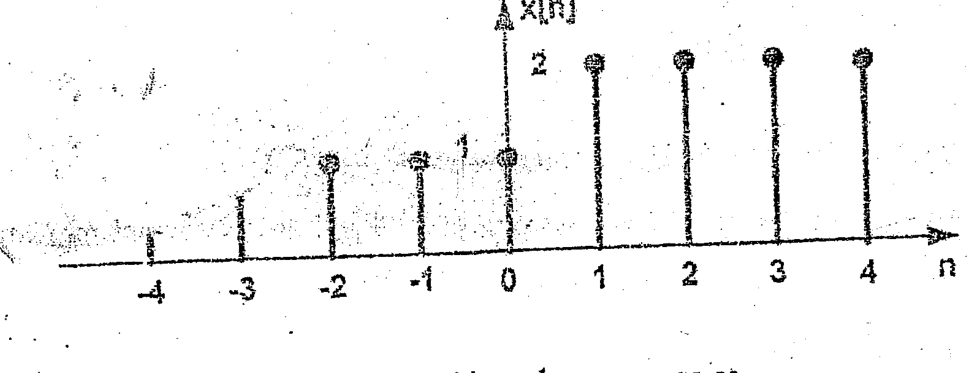
\includegraphics[width=4in]{images/dsap_71shr_stem.png}

      \item Define and plot a discrete time unit step signal. Explain its relation with the unit impulse signal. \hfill [1+2] (\bo{73 Ch})
    \end{enumerate}

  \subsection{Energy / power signals and periodicity}
    \begin{enumerate}[topsep=0pt, noitemsep]
      \item Define (compare) energy and power signal, and determine whether the given signal is periodic (find its fundamental period).
        \lb $x[n]=\cos(2\pi n/5)+\sin(\pi n/3)$ \hfill [2+2] (\bo{79 Bh, 69 Ch})
        \lb $x[n]=e^{j(\pi n/3+\pi/4)}$ \hfill [2+2] (74 Ash)
        \lb $x[n]=e^{j(\pi n/2+4\pi/7)}$ (energy or power?) \hfill [2+2] (79 Ba)
        \lb $x[n]=u[n]$ and $x[n]=\delta[n]$: energy or power type? \hfill [2+3] (72 Ka)
        \lb Power Vs energy signal; Fourier Series Vs Fourier Transform. \hfill [3+4] (\bo{75 Ch})

      \item Determine whether the signal is periodic; if periodic, state its periodic/fundamental time.
        \lb $x[n]=e^{j\pi n/16}\cos(n\pi/17)$ \hfill [5] (\bo{80 Bh})
        \lb (a) $\sin(n\pi)+\cos(n\pi)$ (b) $\sin(3n\pi/5)+\cos(4n\pi/7)$ \hfill [2+2] (80 Ba)
        \lb $x[n]=\cos(\pi n/2)\cos(\pi n/4)$ \hfill [4] (\bo{78 Bh})
        \lb (i) $\cos(\pi n^2/8)$ (ii) $\cos(n/2)\cos(\pi n/4)$ \hfill [3] (\bo{70 Ch})
    \end{enumerate}

  \subsection{System properties (linearity, time-invariance, causality, stability)}
    \begin{enumerate}[topsep=0pt, noitemsep]
      \item A DT system is given by $y(n)=\sum_{k=0}^{n}x(k)$; check whether it is memoryless, time-invariant and stable. \hfill [2+2+2] (\bo{80 Bh})

      \item Determine the given systems: (a) $y[n]=x[-n]$ time-invariant? (b) $y[n]=x[n^2]$ linear? \hfill [5] (\bo{76 Ch})
        \lb (a) $y[n]=y[n-4]+x[n-4]$ time-invariant? (b) $y[n]=x^2[n]$ linear? \hfill [3+3] (\bo{74 Ch})
        \lb (a) $y[n]=x^2[n]$ (b) $y[n]=\cos(\tfrac{5\pi}{8}n+\tfrac{\pi}{4})$: linear or not? \hfill [3+3] (75 Ash)

      \item An LTI system is given by $y(n)=x(n)+e^{a}y(n-1)$; check this system for BIBO stability. \hfill [5] (81 Ba)
    \end{enumerate}

  \subsection{Fourier series/transform of DT signals; convolution}
    \begin{enumerate}[topsep=0pt, noitemsep]
      \item Explain the process of calculating Fourier series coefficients. \hfill [3] (73 Shr) [4] (\bo{72 Ch})

      \item Explain the Fourier transform multiplication property for two sequences. Write Dirichlet conditions for Fourier series. \hfill [4+3] (76 Ash)

      \item Find the output $y(n)$ of an LTI system given its impulse response $h$ and input $x$ (convolution). Representative parameter sets:
        \lb $h(n)=\{5,4,3,2\},\ x(n)=\{1,0,3,2\}$ \hfill [6] (\bo{70 Ch})
        \lb $h(n)=\{1,1,1\},\ x(n)=\{1,1,1,1\}$ \hfill [6] (73 Shr)
        \lb $h[n]=(1/2)^n\{u[n+2]-u[n-2]\},\ x[n]=\{2,1,0,-1,4\}$ \hfill [5] (79 Ba)
        \lb $h[n]=(1/2)^n\{u[n+2]-u[n-2]\},\ x[n]=\{2,1,0.5,-1\}$ \hfill [3+2] (74 Ash)
        \lb $h[n]=(1/3)^n\{u[n+1]-u[n-2]\},\ x[n]=\{2,1,0.5,3\}$ \hfill [5] (72 Ka)
        \lb $h[n]=u[n]-u[n-4],\ x[n]=(1/2)^n u[n]$ \hfill [5] (\bo{78 Bh})
        \lb $h[n]=(1/3)^n u[n],\ x[n]=5e^{j\pi n/2}$ \hfill [4] (\bo{70 Ch})
        \lb $h[n]=(1/2)^n u[n],\ x[n]=5e^{j\pi n/3}$ \hfill [4/5] (72 Ka, \bo{80 Ba})
        \lb $h[n]=(1/2)^n u[n],\ x[n]=10-5\sin(\pi n/2)+20\cos(\pi n)$ \hfill [3+7] (73 Shr)
        \lb $h[n]=(1/3)^n u[n-1]/\,\dots,\ x[n]=u[n+1]-u[n-4]$ \hfill [6] (\bo{76 Ch})
        \lb $x[n]=\delta[n]+2\delta[n-1]-\delta[n-3],\ h[n]=2\delta[n+1]+2\delta[n-1]$ \hfill [5] (\bo{79 Bh})
        \lb $h(n)=\{1,3,2,-1,1\},\ x(n)=2\delta(n)-\delta(n-1)$ \hfill [6] (\bo{71 Ch})
        \lb $h(n)=(1/3)^n u[n],\ x(n)=\{2,1,0.5,3\}$ etc.

      \item LTI output from table values (convolution) --- $x[-2]=0.5,x[0]=1,x[1]=0.75,x[3]=0.5$; $n[0]=1,n[1]=0.75,n[2]=0.5$; verify. \hfill [6] (\bo{73 Ch})
        \lb $h[-2]=3,h[0]=2,h[1]=1,\ x[n]=2^n,\ -1\le n\le3$; check. \hfill [5+2] (\bo{75 Ch})
        \lb $h[-2]=1,h[0]=2,h[1]=3,\ x[0]=1/2,x[2]=2,x[3]=3$; check. \hfill [3+2] (\bo{72 Ch})

      \item Illustrate the significance of convolution summation in digital signal analysis and compute the convolution $h(n)=\{1,0,1\},\ x(n)=\{1,-2,-2,3,4\}$. \hfill [2+4] (70 Ash)
        \lb Find the convolution $x[n]=a^n u[-n],\ 0<a<1,\ h[n]=u[n]$. \hfill [6] (76 Ash)
    \end{enumerate}

\pagebreak
%=======================================================================
\section{Z-Transform}
\begin{center}(4 Hours)\end{center}

  \subsection{ROC --- definition and properties}
    \begin{enumerate}[topsep=0pt, noitemsep]
      \item Define ROC / state and explain the properties of Region of Convergence (and locate the ROC of a signal). \hfill [1--3] (\bo{80 Bh, 73 Ch, 72 Ch}, 79 Ba, 72 Ka, 71 Shr)
        \lb Properties of ROC + locate ROC of $x[n]=(-1/3)^n u[n]-(1/3)^n u[-n-1]$ \hfill [2+4] (\bo{70 Ch})
        \lb Properties of ROC + locate ROC of $x[n]=(0.6)^n u[n]+(0.25)^n u[n]$ \hfill [3+6] (75 Ash)
        \lb Properties of ROC + locate ROC of $x[n]=(0.1)^n u[n]+(0.3)^n u[-n-1]$ \hfill [4+6] (\bo{75 Ch})
        \lb List properties of ROC + Z-transform \& locate ROC of $x[n]=(-1/3)^n u[n]-(1/3)^n u[-n-1]$ \hfill [2+4] (70 Ash)
    \end{enumerate}

  \subsection{Properties of Z-transform (convolution, time-shift)}
    \begin{enumerate}[topsep=0pt, noitemsep]
      \item State the convolution property of Z-transform (and derive it). \hfill [3+3/3+6] (76 Ash, 72 Ka, 70 Ash)
      \item Derive the time shifting property of Z-transform. \hfill [3+3] (\bo{69 Ch})
    \end{enumerate}

  \subsection{Inverse Z-transform (partial fraction / long division)}
    \begin{enumerate}[topsep=0pt, noitemsep]
      \item Determine the inverse Z-transform (state the ROC region as given):
        \lb $H(z)=\dfrac{1+2z^{-1}+z^{-2}}{1-0.75z^{-1}+0.125z^{-2}},\ 0.25<|z|<0.5$ \hfill [1+6] (\bo{80 Bh})
        \lb $X(z)=\dfrac{1}{1-0.8z^{-1}+0.12z^{-2}}$ for $|z|>0.6$, $|z|<0.2$, $0.2<|z|<0.6$ \hfill [2+2+3] (81 Ba)
        \lb $X(z)=\dfrac{1+2z^{-1}+z^{-2}}{1-1.5z^{-1}+0.5z^{-2}},\ |z|>1$ \hfill [1+5] (80 Ba)
        \lb $X(z)=\dfrac{2z^4+2z^3-3z+2}{z^2-1.5z-1},\ |z|<0.5$ (partial fraction) \hfill [6] (\bo{79 Bh})
        \lb $H(z)=\dfrac{z}{3z^2-4z+1},\ \tfrac13<|z|<1$ (partial fraction) \hfill [1+5] (79 Ba)
        \lb $X(z)=\dfrac{z^3+z^2+1.5z+0.5}{z^3+1.5z^2+0.5z},\ |z|<1/2$ \hfill [1+5] (\bo{78 Bh})
        \lb $X(z)=\dfrac{z^4+5z^3-3z+4}{z^2-1.5z-1},\ |z|<0.5$ \hfill [2+6] (\bo{76 Ch})
        \lb $X(z)=\dfrac{z}{(z-0.6)(z+0.5)^2},\ |z|>0.6$ \hfill [3+6] (76 Ash)
        \lb $X(z)=z^2\big[1-\tfrac32 z^{-1}\big](1+z^{-1})(1-z^{-1})$ \hfill [3+3] (74 Ash)
        \lb $X(z)=\dfrac{2z^2+2z^2+3z+5}{z^2-0.1z-0.2},\ |z|<0.4$ \hfill [1+3+5] (\bo{74 Ch, 73 Ch})
        \lb $X(z)=\dfrac{z}{(z-0.4)(z+1.5)^2},\ |z|<0.4$ \hfill [1+5] (73 Shr)
        \lb $X(z)=\dfrac{1}{(z-0.5)(z+2)}$: $0.5<|z|<2$, $|z|<0.5$, $|z|>2$ \hfill [1+5] (\bo{71 Ch})
        \lb $X(z)=\dfrac{1+2z^{-1}+z^{-2}}{1+1.5z^{-1}+0.5z^{-2}},\ |z|>1$ \hfill [6] (71 Shr)
        \lb $X(z)=\dfrac{z}{(z-1)(z-2)^2},\ |z|<1$ \hfill [1+5] (70 Ash)
    \end{enumerate}

\pagebreak
%=======================================================================
\section{Analysis of LTI Systems in Frequency Domain}
\begin{center}(6 Hours)\end{center}

  \subsection{Pole--zero plot and magnitude/phase response}
    \begin{enumerate}[topsep=0pt, noitemsep]
      \item Plot the pole-zero in the z-plane and draw the magnitude response (not to scale) of the system described by the given difference equation:
        \lb $y(n)=x(n)+0.8x(n-1)+0.8x(n-2)+0.49y(n-2)$ \hfill [3+7] (\bo{80 Bh})
        \lb $y(n)=0.67x(n)-0.3x(n-1)+2.75y(n-1)$ \hfill [3+7] (81 Ba); phase response \hfill [2+8] (76 Ash)
        \lb $y[n]-0.35y[n-1]+0.25y[n-2]=x[n]-0.75x[n-1]$ \hfill [3+7] (\bo{79 Bh})
        \lb $y[n]-0.3y[n-1]+0.2y[n-2]=x[n]-0.5x[n-1]$ \hfill [3+7] (79 Ba)
        \lb $y[n]-0.4y[n-1]+0.25y[n-2]=x[n]-0.4x[n-1]$ \hfill [2+4] (\bo{78 Bh})
        \lb $y[n]-0.4y[n-1]+0.2y[n-2]=x[n]+0.5x[n-1]+0.6x[n-2]+0.8x[n-3]$ \hfill [3+7] (74 Ash)
        \lb $y[n]-0.5y[n-1]+0.3y[n-2]=x[n]+0.7x[n-1]$ \hfill [6] (72 Ka)
        \lb $y[n]-0.4y[n-1]+0.1y[n-2]=x[n]+0.6x[n-1]$ \hfill [2+4] (\bo{72 Ch})
        \lb $y[n]-0.3y[n-1]+0.225y[n-2]=x[n]+0.5x[n-1]$ \hfill [6] (\bo{70 Ch})
        \lb $y[n]-0.4y[n-1]+0.2y[n-2]=x[n]+0.1x[n-1]-0.06x[n-2]$ \hfill [2+2+6] (\bo{69 Ch})
        \lb $y(n)-0.3y(n-1)=2x(n-2)+0.7x(n-1)+4x(n)$ \hfill [2+7] (\bo{75 Ch})

      \item Map the poles and zeros in the z-plane and plot the magnitude response for a system with given pole/zero locations:
        \lb poles $0.45\pm j1.6$, zeros $0.58\pm j2.06$ \hfill [4+6] (80 Ba)
        \lb poles $0.45\pm j1.06$, zeros $0.58\pm j2.06$ \hfill [2+6/2+8] (\bo{76 Ch}, 75 Ash)
        \lb poles $0.45-0.77i$ and $-2\pm0.3i$ \hfill [2+8] (\bo{74 Ch})
        \lb poles $0.45+0.77i$, $2\pm0.7i$, zeros $1.2\pm0.43i$ \hfill [2+8] (\bo{73 Ch})
        \lb poles $0.45+0.77i$, $-2\pm0.3i$, zeros $1.2\pm3i$ \hfill [2+8] (\bo{71 Ch})
        \lb $y(n)=x(n)+x(n-2)$: poles/zeros + magnitude + causal \& stable? \hfill [2+6+2] (70 Ash)
    \end{enumerate}

  \subsection{FIR vs IIR, LCCDE, linear phase, stability/causality}
    \begin{enumerate}[topsep=0pt, noitemsep]
      \item Differentiate between FIR system and IIR system. \hfill [4+6] (80 Ba)
      \item State linear constant coefficient difference equation and the corresponding system function. \hfill [3+7] (73 Shr) [2+3+5] (71 Shr)
      \item Determine the zero-input response for the second order system $y[n]-3y[n-1]-4y[n-2]=x[n]$. \hfill [4] (\bo{78 Bh})
      \item Describe stability and causality characteristics of an LTI system in terms of Impulse Response and ROC of its transfer function with examples. \hfill [4+3] (76 Ash) [4] (\bo{72 Ch})
      \item What is the condition satisfied by a linear phase FIR filter? Show that the filter with $h(n)=\{-1,0,1\}$ is a linear phase filter. \hfill [2+4] (70 Ash)
    \end{enumerate}

\pagebreak
%=======================================================================
\section{Discrete Filter Structures}
\begin{center}(8 Hours)\end{center}

  \subsection{Direct form and cascade realizations}
    \begin{enumerate}[topsep=0pt, noitemsep]
      \item Obtain the Direct Form I and Direct Form II realization of the given system:
        \lb $y[n]=-0.25y[n-2]+x[n]+0.4x[n-1]+0.5x[n-2]$ \hfill [2+2] (\bo{79 Bh})
        \lb $y[n]-0.75y[n-1]-0.25y[n-2]=x[n]+0.5x[n-1]$ \hfill [4] (79 Ba)
        \lb $3y[n]+y[n-1]+2y[n-4]=2x[n]+x[n-3]$ \hfill [5] (\bo{74 Ch})
        \lb $y(n)=-0.1y(n-1)+0.2y(n-2)+3x(n)+3.6x(n-2)+0.6x(n-2)$ \hfill [5] (\bo{72 Ch})
        \lb Direct Form II only: $y(n)=-0.1y(n-1)+0.72y(n-2)+0.7x(n)-0.252x(n-2)$ \hfill [4] (72 Ka, \bo{69 Ch})

      \item Realize the given system in cascade form of second-order sections (signal flow graph):
        \lb $H(z)=10(1-0.25z^{-1})(1-0.667z^{-1})(1+2z^{-1})/[(1-0.75z^{-1})(1-0.125z^{-1})(1-(0.5+j0.5)z^{-1})(1-(0.5-j0.5)z^{-1})]$ \hfill [5] (81 Ba)
        \lb $H(z)=\{(1-0.4z^{-1})(1+0.2z^{-1})(1-0.3e^{j\pi/6}z^{-1})(1-0.3e^{-j\pi/6}z^{-1})\}/\{(1-0.5e^{j\pi/3}z^{-1})(1-0.5e^{-j\pi/3}z^{-1})(1+0.7e^{j\pi/4}z^{-1})(1+0.7e^{-j\pi/4}z^{-1})\}$ \hfill [4] (80 Ba)
        \lb Similar 2nd-order cascade with $e^{j2n\pi/5}$ etc. \hfill [4] (\bo{76 Ch})
        \lb $y[n]-\tfrac34 y[n-1]+\tfrac18 y[n-2]-x[n]-2x[n-1]=0$ \hfill [4] (\bo{70 Ch})
    \end{enumerate}

  \subsection{Lattice / lattice-ladder structures}
    \begin{enumerate}[topsep=0pt, noitemsep]
      \item Draw the lattice (or lattice-ladder) structure for the given system function (and check stability where asked):
        \lb $H(z)=1/(1-0.2z^{-1}+0.4z^{-2}+0.6z^{-3})$ \hfill [10] (\bo{80 Bh})
        \lb FIR $H(z)=1+(13/24)z^{-1}+(5/8)z^{-2}+(1/3)z^{-3}$, check stability \hfill [5] (81 Ba); Direct + Lattice \hfill [3+7] (\bo{78 Bh})
        \lb lattice-ladder $H(z)=(2-0.7z^{-1}+0.5z^{-2})/(1-0.3z^{-1}+0.25z^{-2})$ \hfill [6] (80 Ba)
        \lb lattice-ladder $H(z)=(1-0.4z^{-1}+0.25z^{-2})/(1-0.3z^{-1}+0.5z^{-2})$, stability \hfill [6+1] (79 Ba)
        \lb lattice-ladder $H(z)=(0.5-2z^{-1}+3z^{-2})/(1-0.5z^{-1}-0.7z^{-2}+0.3z^{-3})$ \hfill [6+4] (\bo{76 Ch})
        \lb lattice-ladder $H(z)=(0.7-1.5z^{-1}+0.5z^{-2})/(1-0.5z^{-1}-0.7z^{-2}+0.3z^{-3})$ \hfill [6+3] (76 Ash)
        \lb $H=1/(3+(39/24)z^{-1}+(15/8)z^{-2}+(3/9)z^{-3})$; also represent $5/8,-5/8$ in sign-magnitude, 1's and 2's complement \hfill [7+3] (75 Ash)
        \lb $H(t)=1/(1+\tfrac23 z^{-1}+\tfrac58 z^{-2}+\tfrac23 z^{-3}+z^{-4})$ \hfill [9] (\bo{75 Ch})
        \lb FIR $H(z)=1+2z^{-1}+z^{-2}$ \hfill [5] (\bo{72 Ch})
        \lb FIR $H(z)=A_3(z)=1+(52/96)z^{-1}+(25/40)z^{-2}+(1/3)z^{-3}$ \hfill [5] (\bo{74 Ch})
        \lb Direct + Lattice, FIR $H(z)=1+0.7z^{-1}+1.2z^{-2}-z^{-3}$ \hfill [3+7] (74 Ash)
        \lb Direct + Lattice, $H(z)=2+1.8z^{-1}-1.6z^{-2}+z^{-3}$ \hfill [3+7] (73 Shr)
        \lb Direct + Lattice, $H(z)=1+\tfrac13 z^{-1}+\tfrac98 z^{-2}+\tfrac43 z^{-3}+z^{-4}$ over denominator \hfill [10] (\bo{73 Ch})
        \lb FIR $H(z)=1+2z^{-1}-3z^{-2}+4z^{-3}$ \hfill [6] (72 Ka, \bo{69 Ch})
        \lb FIR $H(z)=1+3.1z^{-1}+5.5z^{-2}+4.2z^{-3}+2.3z^{-4}$ \hfill [6] (\bo{70 Ch})
        \lb IIR $H(z)=1/(1-0.01z^{-1}-0.23z^{-2}+0.5z^{-3})$, stability \hfill [4+2+1] (\bo{71 Ch})
        \lb pole-zero $H(z)=(0.5+2z^{-1}+0.6z^{-2})/(1-0.3z^{-1}+0.4z^{-2})$ \hfill [6] (70 Ash)

      \item Given a 3-stage lattice filter for an all-zero/all-pole polynomial with coefficients $K_1=1/4,K_2=1/2,K_3=1/3$: obtain the system function and FIR filter coefficients. \hfill [6] (\bo{79 Bh}) [5] (71 Shr)
    \end{enumerate}

  \subsection{Quantization effects, limit cycles, dead band}
    \begin{enumerate}[topsep=0pt, noitemsep]
      \item What is the limit cycle effect in a recursive system? Describe with an example showing how it occurs. \hfill [3] (\bo{71 Ch}) [1+3] (70 Ash)
      \item What is the importance of quantization in DSP? Which is better, rounding or truncation? Explain limit cycles in a recursive system and define dead band. \hfill [1+1+2+1] (71 Shr)
    \end{enumerate}

\pagebreak
%=======================================================================
\section{FIR Filter Design}
\begin{center}(6 Hours)\end{center}

  \subsection{Window method and Gibbs phenomenon}
    \begin{enumerate}[topsep=0pt, noitemsep]
      \item Describe how a digital FIR filter is designed by the window method (discuss characteristics of different window functions). \hfill [4+4] (\bo{70 Ch}) [5+3] (\bo{72 Ch})
      \item Design a symmetric/linear-phase FIR LPF using a suitable window:
        \lb $H_d(\omega)=e^{-j\omega\tau}$, $|\omega|\le\omega_c$; length 7, $\omega_c=1$ rad; Hanning window \hfill [10] (\bo{80 Bh})
        \lb $\omega_p=0.2\pi,\ \omega_s=0.45\pi,\ \alpha_s=51$ dB, any window \hfill [5+3] (79 Ba)
        \lb $\omega_p=0.3\pi,\ \omega_s=0.5\pi,\ \alpha_s=40$ dB, suitable window \hfill [8] (\bo{71 Ch, 69 Ch})
        \lb first six coefficients; $\omega_p=0.2\pi,\ \omega_s=0.5\pi,\ \alpha_s=41$ dB (Why is Kaiser better?) \hfill [2+6] (74 Ash)
        \lb Hanning window; $\omega_p=0.25\pi,\ \omega_s=0.35\pi$, main-lobe width $8\pi/M$ \hfill [9] (70 Ash)
      \item Explain Gibbs phenomenon / oscillation and how it arises with the rectangular window (and how it can be minimized). \hfill [3+3/5/6] (81 Ba, 80 Ba, 73 Shr, 71 Shr)
    \end{enumerate}

  \subsection{Kaiser window design}
    \begin{enumerate}[topsep=0pt, noitemsep]
      \item Design a linear phase FIR filter using the Kaiser window for the given specifications (determine ripple, $\beta$, and length $M+1$ where asked):
        \lb $0.99\le|H|\le1.01,\ 0\le|w|\le0.3\pi$; $|H|\le0.01,\ 0.35\pi\le|w|\le\pi$ \hfill [10] (81 Ba)
        \lb $|H|\le0.01,\ 0.21\pi\le|\omega|\le\pi$; $0.95\le|H|\le1.05,\ 0\le|\omega|\le0.19\pi$ (ripple, atten, length) \hfill [2+2+2] (\bo{80 Bh})
        \lb $0.99\le|H|\le1.01,\ 0\le w\le0.016\pi$; $|H|\le0.01,\ 0.08\pi\le w\le2\pi$ \hfill [2+8] (80 Ba)
        \lb $0.899\le|H|\le1,\ |w|\le0.2\pi$; $|H|\le0.01,\ 0.4\pi\le w\le\pi$ \hfill [2+8] (\bo{79 Bh})
        \lb $|H|\le0.01,\ 0\le w\le0.25\pi$; $0.95\le|H|\le1.05,\ 0.35\pi\le w\le0.6\pi$; $|H|\le0.01,\ 0.65\pi\le w\le\pi$ \hfill [8] (\bo{78 Bh}); with min length $M+1$ and $\beta$ \hfill [9+3] (\bo{74 Ch})
        \lb $0.99\le|H|\le1.01,\ 0\le w\le0.19\pi$; $|H|\le0.01,\ 0.21\pi\le w\le\pi$ (+ optimum-filter flowchart) \hfill [8+4] (75 Ash) [6+8] (72 Ka)
        \lb $0.99\le|H|\le1.01,\ 0\le w\le0.16\pi$; $|H|\le0.01,\ 0.18\pi\le w\le2\pi$ (+ Remez flowchart) \hfill [2+4+4] (76 Ash)
        \lb $0.98\le|H|\le1.02,\ 0\le w\le0.9\pi$; $|H|\le0.01,\ 0.14\pi\le w\le\pi$ \hfill [8] (\bo{73 Ch})
    \end{enumerate}

  \subsection{Optimum filter / Remez exchange algorithm}
    \begin{enumerate}[topsep=0pt, noitemsep]
      \item What is an optimum filter? Show the mathematical expression / draw the flowchart of the Remez exchange algorithm for FIR filter design (with derivation where asked). \hfill [1+5/1+6/2+6/7/9] (\bo{75 Ch, 72 Ch, 70 Ch, 69 Ch}, 76 Ash, 73 Shr, 71 Shr, \bo{73 Ch})
        \lb Describe the Remez exchange algorithm with flowchart. \hfill [5/1+6] (\bo{79 Bh}, 79 Ba)
    \end{enumerate}

\pagebreak
%=======================================================================
\section{IIR Filter Design}
\begin{center}(6 Hours)\end{center}

  \subsection{Bilinear transformation (Butterworth)}
    \begin{enumerate}[topsep=0pt, noitemsep]
      \item Design a digital IIR/Butterworth LPF using the bilinear transformation method for the given specifications:
        \lb $0.9\le|H|\le1,\ 0\le w\le\pi/2$; $|H|\le0.2,\ 3\pi/4\le w\le\pi$; $f_s=1$ \hfill [12] (\bo{80 Bh})
        \lb $0.6\le|H|\le1,\ 0\le\omega\le0.35\pi$; $|H|\le0.1,\ 0.7\pi\le\omega\le\pi$; $T=0.1$ s (bilinear Vs impulse invariance) \hfill [2+10] (81 Ba)
        \lb passband edge $0.26\pi$, deviation $0.99$ dB; max gain $-14.99$ dB at $0.58\pi$; $f_s=0.5$ \hfill [11] (80 Ba)
        \lb $W_p=0.25\pi,W_s=0.55\pi,\delta_p=0.11,\delta_s=0.21,f_s=0.5$; then convert to HPF $W'_p=0.45\pi$ \hfill [11+4] (\bo{79 Bh}, \bo{71 Ch}, \bo{69 Ch})
        \lb passband edge $0.24\pi$, deviation $0.98$ dB; max gain $-14.95$ dB at $0.57\pi$; $f_s=0.5$ (compare with impulse invariance) \hfill [11+3] (79 Ba)
        \lb $0.99\le|H|\le1.01\dots$ (specs) \hfill (various)
        \lb $0.8\le|H|\le1,\ 0\le W\le0.2\pi$; $|H|\le0.2,\ 0.6\pi\le W\le\pi$ \hfill [10] (\bo{75 Ch, 70 Ch})
        \lb $0.707\le|H|\le1,\ 0\le w\le\pi/2$; $|H|\le0.2,\ 3\pi/4\le w\le\pi$; $T=1$ s (realize convenient form) \hfill [11+4] (\bo{73 Ch})
        \lb $0.89125\le|H|\le1,\ 0\le\omega\le0.2\pi$; $|H|\le0.17783,\ 0.3\pi\le\omega\le\pi$ \hfill [12] (73 Shr)
        \lb passband peak-to-peak ripple $\le1$ dB, passband edge $1.2$ kHz; stopband atten $\ge40$ dB, edge $2.5$ kHz; $f_s=8$ kHz \hfill [10] (\bo{76 Ch})
        \lb passband const $0.7$ dB below $0.15\pi$; stopband $\ge14$ dB, $0.6\pi$ to $\pi$ \hfill [12] (75 Ash, \bo{74 Ch})
        \lb $\omega_p=0.22\pi,\omega_s=0.54\pi,\delta_p=0.11,\delta_s=0.22,f_s=0.5$ \hfill [12] (76 Ash)
        \lb $\omega_p=0.27\pi,\omega_s=0.58\pi,\delta_p=0.11,\delta_s=0.21,f_s=0.5$ \hfill [15] (74 Ash)
        \lb passband edge $0.25\pi$, deviation $1$ dB; max gain $-15$ dB at $0.45\pi$; $f_s=1$ \hfill [15] (72 Ka)
        \lb passband edge $0.2\pi$, deviation $1$ dB; max gain $-15$ dB at $0.4\pi$; $f_s=1$ \hfill [15] (71 Shr)
    \end{enumerate}

  \subsection{Impulse invariance method}
    \begin{enumerate}[topsep=0pt, noitemsep]
      \item Design a Butterworth LPF using the Impulse Invariance Method:
        \lb passband/stopband $200$ Hz / $500$ Hz, atten $5$ dB / $12$ dB, $f_s=5000$ Hz; explain pre-warping and why it is necessary \hfill [12+3] (\bo{78 Bh})
        \lb (+) of bilinear over impulse invariance; $200$/$500$ Hz, $-5$/$-12$ dB, $f_s=5$ kHz (IIM) \hfill [3+12] (\bo{72 Ch})
        \lb passband edge $0.2\pi$, deviation $0.5$ dB; max gain $-15$ dB at $0.35\pi$; $f_s=1$ \hfill [13] (70 Ash)
      \item Explain briefly the bilinear transformation method of IIR filter design / its advantages over impulse invariance. \hfill [3] (73 Shr)
    \end{enumerate}

  \subsection{Spectral (digital domain) transformation}
    \begin{enumerate}[topsep=0pt, noitemsep]
      \item Describe digital-domain spectral transformation features and parameters for low-pass to high-pass conversion in IIR filter design. \hfill [4] (80 Ba)
      \item Why is spectral transformation required? \hfill [2] (70 Ash)
      \item A digital LPF with $w_c=0.2575\pi$ is $H(z)=(0.1+0.4z^{-1})/(1-0.6z^{-1}+0.1z^{-2})$; design a digital HPF with $w'_c=0.3567\pi$. \hfill [5] (\bo{70 Ch})
    \end{enumerate}

\pagebreak
%=======================================================================
\section{Discrete Fourier Transform (DFT and FFT)}
\begin{center}(7 Hours)\end{center}

  \subsection{DFT --- definition, properties, DFT vs DTFT}
    \begin{enumerate}[topsep=0pt, noitemsep]
      \item Why do we need DFT / FFT (although we have DTFT)? Differentiate between DFT and DTFT; write the computational complexity of DFT and FFT. \hfill [2--2+5] (\bo{79 Bh, 78 Bh, 71 Ch}, 79 Ba, 80 Ba)
      \item State and prove the circular convolution property of DFT. \hfill [2+2+4] (\bo{70 Ch})
      \item Define zero padding / padding zones. \hfill [1] (\bo{74 Ch, 74 Ash, 70 Ch})
    \end{enumerate}

  \subsection{FFT computation (DIT / DIF)}
    \begin{enumerate}[topsep=0pt, noitemsep]
      \item Find the $N$-point DFT of the given sequence using the DIT-FFT or DIF-FFT algorithm (draw the butterfly diagram where asked):
        \lb 8-pt DIF, $x(n)=\{2,1,2,1,1,2,1,2\}$ \hfill [8] (\bo{80 Bh})
        \lb 4-pt DIT, $x(n)=\{2,2,4\}$ (Why DIT-FFT better than direct DFT?) \hfill [2+6] (81 Ba)
        \lb 8-pt DIF, $x[n]=\{1,1,0,0,1,1,2\}$ \hfill [2+6] (80 Ba, \bo{70 Ch})
        \lb 8-pt radix-2 DIT, $x[n]=u[n]-u[n-4]$ / general \hfill [2+6/7] (\bo{79 Bh, 78 Bh})
        \lb 8-pt DIF, $x[n]=\{1,2,4,3,5,-1,3\}$ \hfill [2+6] (79 Ba)
        \lb 8-pt DIF, $x[n]=\{1,2,3,3,5,0,4,6\}$ \hfill [7] (\bo{76 Ch})
        \lb 8-pt DIF, $x[n]=\{1,2,3,3,5,1,4,2\}$ \hfill [2+8] (76 Ash)
        \lb $X(3),X(5)$ of $x[n]=\{1,-2,3,2\}$ (DIT-FFT) \hfill [2+8] (\bo{75 Ch})
        \lb butterfly 8-pt DIT, $x[n]=n+1$ \hfill [3+7] (75 Ash)
        \lb butterfly radix-2 DIF, $X(2),X(1)$ of $x[n]=\{1.5,-1,1.8,0.6,3,1.7\}$ \hfill [3+7] (\bo{74 Ch})
        \lb 8-pt DIF, $x[n]=\{1/2,1/2,1/2,1/2,0,0,0,0\}$ \hfill [7] (74 Ash)
        \lb 8-pt DIF, $x[n]=\{1,-1,3,2,1,1,3,-2\}$ \hfill [2+6] (\bo{73 Ch})
        \lb 8-pt, $x[n]=\{1,-1,2,2,1,1,2,2\}$ \hfill [2+6] (73 Shr)
        \lb DIT, $x[n]=\{1,1,2,4,3,1,2,1\}$ \hfill [8] (\bo{72 Ch})
        \lb 8-pt DIT, $x[n]=\{1,1,0,1,0,1,2\}$ \hfill [7] (72 Ka)
        \lb butterfly $X(7)$, 8-pt DIT, $x(n)=\{1,0,0,0,0,0,0,0\}$ \hfill [2+6] (\bo{71 Ch}, 70 Ash)
        \lb DIT butterfly + spectrum, $x=\{1,1,2,0,1,2,0,1\}$ \hfill [6+2] (71 Shr)
        \lb 8-pt DIF, $x[n]=\{1,1,2,2,1,1,2,1\}$ \hfill [2+7] (\bo{69 Ch})
    \end{enumerate}

  \subsection{Circular convolution (direct and via DFT: $x_3=\text{IDFT}(X_1X_2)$)}
    \begin{enumerate}[topsep=0pt, noitemsep]
      \item Compute the circular convolution of the given sequences (directly or using DFT):
        \lb $x_1=\{1,2,3,1\},\ x_2=\{4,3,2,2\}$ \hfill [6/2+5] (\bo{80 Bh}, 80 Ba)
        \lb $x=\{1,2,4,5\},\ h=\{2,1,6,8\}$ \hfill [6] (81 Ba)
        \lb $x_1=\{1,-1,-2,3,-1\},\ x_2=\{1,2,3\}$ \hfill [7] (79 Ba)
        \lb $x_1=\{2,1,2,1\},\ x_2=\{1,2,3,4\}$ \hfill [2+6] (\bo{78 Bh})
        \lb $x_1=\{1,2,-1,1\},\ x_2=\{1,3,5,7\}$ \hfill [1+5] (75 Ash)
        \lb linear Vs circular; $X_1=\{0,0,1,1\},\ X_2=\{1,1,1,1\}$ \hfill [3+7] (\bo{75 Ch})
        \lb linear conv via circular with zero padding; $x=\{1,1,1,1\},\ h=\{2,3\}$ \hfill [1+5] (\bo{74 Ch})
        \lb $h(n)=\{1,2,1,-1,1\},\ x=\{1,2,3,1\}$ \hfill [7] (\bo{72 Ch})
        \lb circular conv; $x=\{1,2\},\ y=u[n]-u[n-4]$ \hfill [2+5] (\bo{71 Ch}, 70 Ash)

      \item Find $x_3[n]$ if $X_3(k)=X_1(k)X_2(k)$ (product of DFTs $\Rightarrow$ circular convolution):
        \lb 4-pt: $x_1=\{1,2,-2\},\ x_2=\{1,2,3,-1\}$ \hfill [5/6] (\bo{76 Ch, 69 Ch})
        \lb 5-pt: $x_1=\{1,-2,5,1,2\},\ x_2=\{1,2,-3,-2\}$ \hfill [7] (\bo{73 Ch})
        \lb 5-pt: $x_1=\{1,-2,2,1,4\},\ x_2=\{2,1,-3,-1\}$ \hfill [7] (73 Shr)
        \lb $x_1=\{1,2,4\},\ x_2=\{-1,2,3,1\}$ \hfill [2+6] (72 Ka)
        \lb $x_1=\{1,0,0,1\},\ x_2=\{2,0,2\}$ \hfill [7] (\bo{79 Bh})
        \lb 5-pt: $x_1=\{1,2,0,1,-2\},\ x_2=\{1,0,1,1,2\}$ (zero padding) \hfill [1+7] (\bo{74 Ch})
        \lb System $x[n]=\{1,2,3,4\},\ h[n]=\{1,3,5,7\}$; output $y[n]$ if $G[k]=X[k]H[k]$ \hfill [7] (71 Shr)
    \end{enumerate}

\end{document}
